\documentclass[tikz,border=6pt]{standalone}
\usepackage{amsmath,amssymb}
\usetikzlibrary{arrows.meta}

\newcommand{\ITh}{\mathbb{T}_h}
\newcommand{\Lh}{\mathbb{L}_h}
\newcommand{\IT}{\mathbb{T}}
\newcommand{\IL}{\mathbb{L}}

\begin{document}
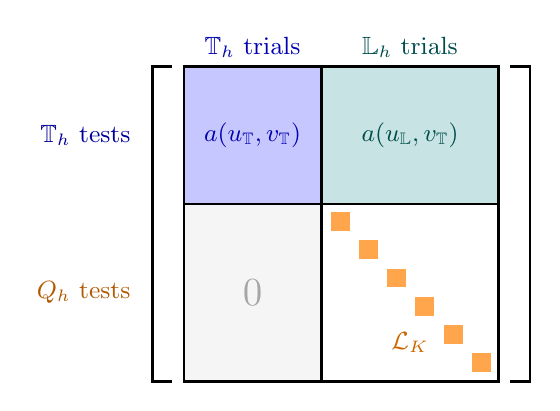
\begin{tikzpicture}[x=1cm,y=1cm,>=Latex]

% colors
\colorlet{cTT}{blue!22}
\colorlet{cTL}{teal!22}
\colorlet{cZero}{black!4}

% geometry
\def\W{4}
\def\H{4}
\def\xs{1.75}
\def\ys{2.25}

% matrix brackets
\draw[line width=1pt]
  (-0.15,0) -- (-0.40,0) -- (-0.40,\H) -- (-0.15,\H);
\draw[line width=1pt]
  (\W+0.15,0) -- (\W+0.40,0) -- (\W+0.40,\H) -- (\W+0.15,\H);

% four main blocks
\fill[cTT] (0,\ys) rectangle (\xs,\H);
\fill[cTL] (\xs,\ys) rectangle (\W,\H);
\fill[cZero] (0,0) rectangle (\xs,\ys);

% block boundaries
\draw[line width=0.8pt] (0,0) rectangle (\W,\H);
\draw[line width=0.8pt] (\xs,0) -- (\xs,\H);
\draw[line width=0.8pt] (0,\ys) -- (\W,\ys);

% "0" block
\node[text=black!35,font=\Large] at ({0.5*\xs},{0.5*\ys}) {$0$};

% diagonal texture inside A_K block
\foreach \x/\y in {
  1.87/1.91,
  2.228/1.552,
  2.586/1.194,
  2.944/0.836,
  3.302/0.478,
  3.660/0.120
}{
  \fill[orange!70] (\x,\y) rectangle ++(0.24,0.24);
}

% row labels
\node[anchor=east,font=\small,text=blue!60!black] at (-0.55,{0.5*(\ys+\H)}) {$\ITh$ tests};
\node[anchor=east,font=\small,text=orange!70!black] at (-0.55,{0.5*\ys}) {$Q_h$ tests};

% column labels
\node[anchor=north,font=\small,text=blue!70!black] at ({0.5*\xs},\H+0.5) {$\ITh$ trials};
\node[anchor=north,font=\small,text=teal!60!black] at ({0.5*(\xs+\W)},\H+0.5) {$\Lh$ trials};

% external block names
\node[font=\small,text=blue!70!black] at ({0.5*\xs},{0.5*(\ys+\H)}) {$a(u_\IT,v_\IT)$};
\node[font=\small,text=teal!60!black] at ({0.5*(\xs+\W)},{0.5*(\ys+\H)}) {$a(u_\IL,v_\IT)$};
\node[font=\small,text=orange!80!black] at ({0.5*(\xs+\W)},{0.22*\ys}) {$\mathcal L_K$};

\end{tikzpicture}
\end{document}
